\documentclass[12pt]{amsart}
\usepackage{amsmath, amssymb, amsthm}
\usepackage[margin=2.5cm]{geometry}
\usepackage{hyperref}
\usepackage{booktabs}
\usepackage{graphicx}

\newtheorem{observation}{Observation}
\newtheorem{derivation}[observation]{Derivation}
\newtheorem{remark}[observation]{Remark}

\title[A response theory for the Riemann zero gas]{A response theory for
the Riemann zero gas:\\ amplitude conservation, a thermal Bragg mirror,
and the two-sum interference}

\author{U\u{g}ur Sezen}
\address{Independent researcher, Istanbul, Turkey}
\email{ugursezen@gmail.com}

\date{\today}

\begin{document}

\begin{abstract}
Two companion notes measured how the local statistics of Riemann zeros
respond to the prime oscillations of the explicit formula: an amplitude
channel $w(\tau)$ and a zero-displacement channel $v(\tau)$, functions of
$\tau = \log p / L$, $L = \log\frac{t}{2\pi}$. Here we organize those
measurements into a coherent response theory. (i) The two channels obey
an \emph{amplitude conservation law}, $\sqrt{w} + (\beta/2)\,v = 1$ with
$\beta/2 \approx 1.07$, whose coefficient agrees with a phase-bookkeeping
ratio within its extrapolation uncertainty;
the law survives an out-of-sample test on unseen primes, a split-half
common-mode test, and a free-exponent test consistent with $k = 2$.
(ii) Extending the measurements to $\tau = 0.61$ shows that $w$
\emph{changes sign} at $\tau_0 = 0.40$ --- the role-crossover of the
companion note --- with response phases that jump from $0$ to $\pi$
without rotating: both channels are real everywhere, consistent with a lossless
(reactive) medium. (iii) A thermal Bragg model explains the crossing: the ideal
mirror sits at the Riemann--Siegel fold $\tau = 1/2$; dressing it with the
\emph{measured} zero-displacement jitter and the measured indirect-channel
plateau brackets the observed zero: the thermal family places it in
$[0.37, 0.41]$ around the measured $0.40$, with unit coherent amplitude
($A \approx 1$) throughout; window-to-window jitter differences absorb
the previously unexplained fixed-$\tau$ scatter. The dephasing scale is the
\emph{standing-wave} factor: the empirical characteristic-function ratio
gives $s = 4.11 \pm 0.04$ against the Gaussian value $4$. (iv) The
structure factor $(1-2\tau)$ is derived in three lines as the pair count
of the folded main sum, vanishing sharply at the fold; pointwise
$|Z|^2$ regressions instead follow the shifted-second-moment family
$\approx 2(1-\tau)$ through and beyond the fold, so that the
complementary \emph{mirror channel} --- measurement minus the direct
pairs --- is a \emph{tent} peaked at the fold --- the approximate functional equation
made audible as an interference channel. (v) The residual variance
decomposes as $\sim 5\%$ unstripped tail, $25$--$45\%$ gap-modulated
prime channel, and a core growing at $0.035$ per unit $L$ --- the CUE
rate at one tenth the amplitude.
\end{abstract}

\maketitle

\section{Introduction}

The first companion note \cite{companion1} measured the joint law of
consecutive-zero gaps and between-zero maxima of Hardy's $Z$-function and
its deviation from CUE characteristic polynomials. The second
\cite{companion2} dissected that deviation into explicit-formula
channels: each prime wave $\cos(t \log p)$ enters the amplitudes at full
weight and splits between a direct amplitude channel $w$ and a
zero-displacement channel $v$, both collapsing onto one-variable laws in
the Berry variable $\tau = \log p / L$ \cite{Berry88}; the channel
decomposition itself is an observable-level counterpart of the hybrid
Euler--Hadamard product \cite{GHK07}. This note asks what \emph{physics} organizes those
curves, and answers with five measured structures: a conservation law, a
sign-crossing, a thermal Bragg model that brackets the crossing's
location, an arithmetic derivation of the structure factor, and the
measurement of the complementary mirror channel. Throughout, the style
of the companions is kept: no closed forms are fitted; every ingredient
is either measured or derived; and every claim is accompanied by the
test that tried to kill it.

Data and conventions are those of \cite{companion1, companion2}: eleven
amplitude windows spanning $t = 1.2\times10^5$ to $2.7\times10^{11}$
(the last from Odlyzko's table of zeros near the $10^{12}$-th
\cite{OdlyzkoTables}), plus six low windows down to $t \approx 1.2\times
10^3$ for the extended-$\tau$ measurements; channels are measured by
linear regression of $\log$(unfolded maxima) and $\log$(unfolded gaps)
on $\cos(t_n \log p), \sin(t_n \log p)$ at gap midpoints, with own-gap
controls for $w$.

\section{The amplitude conservation law}

The second companion's sum rule --- total prime content of unit weight
--- holds at first order in $v$. Its violation
$g = w + \beta v - 1$ is zero at small $\tau$ and grows as
$g \approx 1.17\,v^2$; and $1.17 \approx \beta^2/4$ with
$\beta = 2.14$. The square completes:
\[
w \;=\; \bigl(1 - \tfrac{\beta}{2} v\bigr)^2
\qquad\Longleftrightarrow\qquad
\sqrt{w} + \tfrac{\beta}{2}\, v \;=\; 1 .
\]
The coefficient has an independent motivation: since a gap is the
derivative of the counting function, the displacement response
$U = v/\tau$ is the quadrature partner of the in-phase response $w$,
suggesting $\beta = U(0)/w(0) = 2.01/0.94 \approx 2.14$. The $w(0)$
extrapolation carries the $\pm 5\%$ model uncertainty documented in
\cite{companion2}, and the unconstrained fit below prefers a slope
$1.029 \pm 0.012$ (window-block bootstrap), in mild ($\approx 3\sigma$)
tension with $\beta/2 = 1.07$; we treat the phase-bookkeeping value as
motivated, not derived. (The coarser log--log regression estimate quoted
as $\beta \approx 2.3$ in \cite{companion2} is the same quantity under
a different convention.)

\begin{observation}[Amplitude conservation]
Across $44$ matched $(w, v)$ pairs ($4$ primes $\times$ $11$ windows,
$t$ from $10^5$ to $2.7\times10^{11}$), the free fit gives
$\sqrt{w} = 0.990 - 1.025\,v$ with residual RMS $0.0096$
(slope $1.029 \pm 0.012$ under window-block bootstrap), at the
irreducible per-prime scatter floor; constraining the intercept to $1$
gives slope $1.069 \approx \beta/2$.
\end{observation}

Three attempts to kill the law failed (Figure~\ref{fig:law}).
\emph{Out of sample}: $w$ for $p = 11, 13$ --- never used in deriving the
law, and extending $\tau$ to $0.26$ --- follows the line with RMS
$0.0148$ over $22$ new pairs (with a small one-sided mean offset of
$-0.009$) while $\sqrt{w}$ falls from $0.78$ to $0.45$. \emph{Common mode}: measuring $w$ from even-indexed gaps and $v$
from odd-indexed gaps (independent noise) reproduces the law with
$a = 0.998$, $b = 1.051$, RMS $0.019$ against $0.018$ for same-half
pairs. \emph{Free exponent}: fitting $w = (1 - b v)^k$ jointly is degenerate
along a $(b, k)$ valley (window-block bootstrap spans $k \approx 2$--$4$
with compensating slope), so the exponent alone is determined only at
$O(1)$; conditioning $b$ on the linear law gives $k = 2.01$, and the
discriminating test is the form race: among equal-parameter alternatives
the intensity-unitarity form $w + c v^2 = 1$ fails by a factor $\approx 9$
in RMS.
What is conserved is the \emph{amplitude}, not the intensity: the prime
wave's unit amplitude splits linearly between the transmitted amplitude
$\sqrt{w}$ and the absorbed displacement $(\beta/2) v$.

\begin{figure}[ht]
\centering
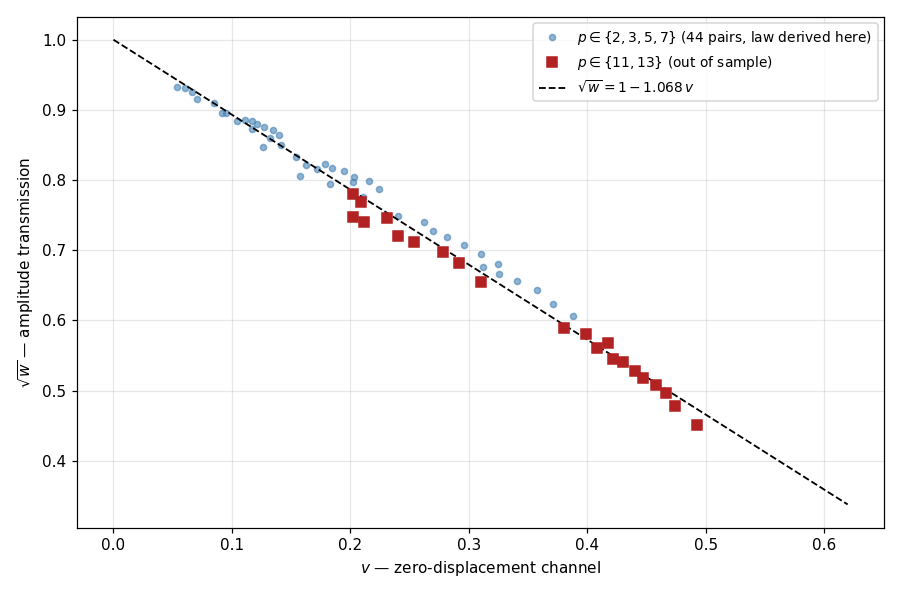
\includegraphics[width=0.8\textwidth]{fig_law_en.png}
\caption{The conservation law. Blue: the $44$ pairs from which the law
was extracted. Red: the $22$ out-of-sample pairs ($p = 11, 13$).}
\label{fig:law}
\end{figure}

\section{The sign crossing and losslessness}

Extending the channel measurements to the primes up to $31$ (eleven
primes) over twelve windows ($132$ points, $\tau$ up to $0.61$) shows that the amplitude channel
does not merely shrink --- it \emph{crosses zero} at
$\tau_0 = 0.40 \pm 0.02$ and settles on a negative plateau
$B = -0.16$: beyond the crossing, peaks are slightly \emph{low} where
the prime wave is high. The crossing coincides with the role-crossover
$\tau^* \approx 0.40$ found by a different method (the exhaustion
analysis of \cite{companion2}), which is thereby identified: $\tau^*$
is the zero of $w$. Two qualifications: the plateau value depends on the
regression basis ($B = -0.16$ for the eleven-prime basis used throughout;
restricted bases give larger values, and more complete bases shrink it
substantially --- its decomposition into genuine indirect response and
basis-transfer systematics is deferred to future work), and the statement
``peaks are low where the wave is high'' holds \emph{at fixed observed
gap} --- without the own-gap controls the unconditional response is
positive.

The response phases are diagnostic. Through the crossing the phase of
$w$ jumps from $\approx 0^\circ$ to $\approx 180^\circ$ with quadrature
components below $3\%$ everywhere; the phase of $v$ stays pinned at
$0^\circ$. A damped resonance would rotate through $\pm 90^\circ$; a
real response that changes sign is the signature of a \emph{lossless}
(conservative, Hermitian) medium. The curtain does not absorb the prime
waves; it redistributes and reflects them --- consistent, at the level
of response theory, with a Hermitian generator underneath. This also
resolves the conservation law's apparent paradox: $w$ reaches zero not
where $v$ would extrapolate the law to closure, but at the sign
crossing; the law describes the below-crossing branch.

\section{The thermal Bragg mirror}

Where should the crossing be? The Riemann--Siegel main sum contains only
$n \le N = \sqrt{t/2\pi}$, i.e.\ $\log n \le L/2$: the amplitude has a
sharp spectral fold at $\tau = 1/2$, and a wave whose period matches two
lattice spacings ($1/\tau = 2$) is precisely the Bragg condition of the
zero lattice. The ideal mirror sits at $\tau = 1/2$; the measured
crossing sits at $0.40$. The shift is thermal.

Model: $w(\tau) = A\,(1 - 2\tau)\, e^{-c \tau^2}\,[\tau < 1/2] + B$,
where $(1-2\tau)$ is the ideal structure factor (derived in
Section~\ref{sec:fold}), $B$ is the indirect (zero-mediated) channel
measured as the beyond-fold plateau, and the Gaussian factor is
Debye--Waller dephasing by the zeros' displacement jitter. The jitter is
\emph{measured}: comparing gap midpoints with the Riemann--von Mangoldt
flow gives $\sigma_u$ per window; in unfolded units it grows from
$0.198$ to $0.272$ across our windows --- the crystal warms
logarithmically, as the classical $S(t)$ variance suggests --- giving
$c = (L \sigma_u)^2/2 = 0.77$--$1.46$, mean $1.17$.

\begin{observation}[The crossing is bracketed]
With $c$ fixed from the measured jitter and $B$ fixed from the measured
plateau, the single remaining parameter fits to $A = 1.03 \approx 1$
(unit coherent amplitude) and the model's zero lands at $\tau = 0.406$
(Figure~\ref{fig:crossing}); with the empirical standing-wave damping,
which fits the full curve best (RMS $0.029$ vs $0.052$), the zero moves
to $0.368$; intermediate damping scales fit equally well and cross at
$0.39$. The thermal family thus brackets the measured crossing within
$[0.37, 0.41]$; no member is simultaneously the best global fit and the
exact crossing, which we attribute to the crude ideal structure factor
and to partial reflection below the Bragg condition.
\end{observation}

Two refinements. First, giving each window its own measured $c(L)$, together with one
fitted overall damping scale, collapses the previously unexplained
fixed-$\tau$, window-to-window scatter of the channel measurements from
$\pm 0.04$ to $\pm 0.003$: the ``secondary variable'' of the companion
note is the window temperature.
Second, the \emph{scale} of the dephasing is consistent with
standing-wave physics: at a Bragg mirror the intracavity field has period
$2k$, so dephasing involves $e^{2 i k u}$ rather than $e^{i k u}$. Measured empirically
--- as the ratio of log characteristic functions of the displacement
series, with no Gaussian assumption --- this gives
\[
s_{\mathrm{eff}} \;=\; \frac{\ln |\langle e^{2 i k u}\rangle|}
{\ln |\langle e^{i k u}\rangle|} \;=\; 4.11 \pm 0.04 ,
\]
the Gaussian value $4$ dressed by the measured sub-Gaussian displacement
statistics (excess kurtosis $-0.3$ to $-0.5$ --- level repulsion
suppressing the tails). Replacing the Gaussian factor by the empirical
$|\langle e^{2iku}\rangle|$ halves the model residual (RMS
$0.074 \to 0.052 \to 0.029$ for no damping, naive, and standing-wave
damping respectively). Two honest caveats: the ratio $s_{\mathrm{eff}}$
is largely a measurement of the near-Gaussianity of $u$ (any
near-Gaussian series gives $\approx 4$), and damping at intermediate
scales (e.g.\ $1.5k$) fits the $w$ curve equally well while crossing at
$0.39$; so the standing-wave scale is \emph{consistent} rather than
demonstrated, with partial reflection below the Bragg condition the
natural interpolation --- an open refinement.

\begin{figure}[ht]
\centering
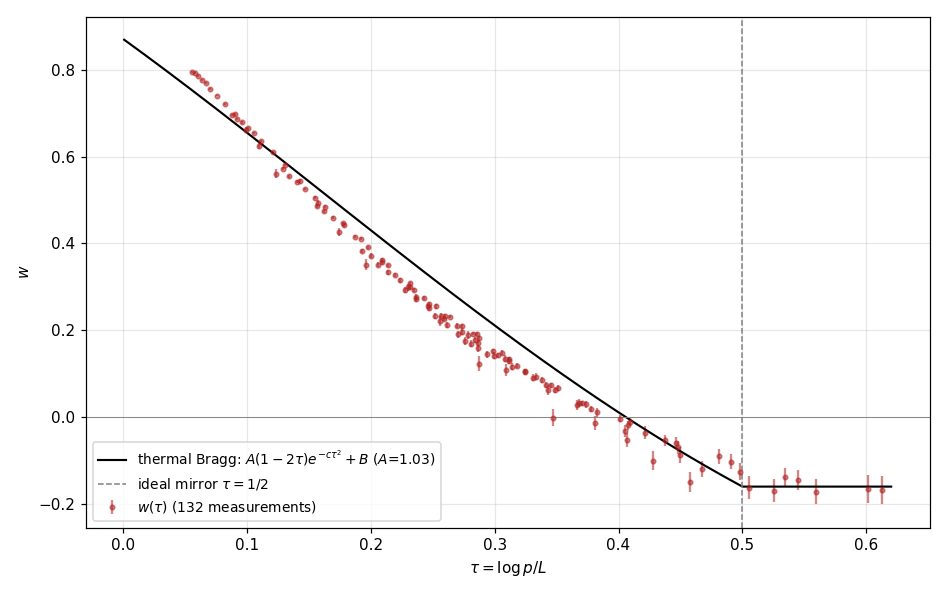
\includegraphics[width=0.82\textwidth]{fig_crossing_en.png}
\caption{The sign crossing and the thermal Bragg model with $c$ from the
measured jitter, $B$ from the measured plateau, and $A = 1.03$ the only
fitted number.}
\label{fig:crossing}
\end{figure}

\section{The structure factor, derived}\label{sec:fold}

\begin{derivation}
Write $Z = 2\sum_{n \le N} n^{-1/2} \cos\phi_n$,
$\phi_n = \theta(t) - t \log n$. In $|Z|^2$ the frequency $\log p$ is
produced exactly by the pairs $(m, mp)$ with $mp \le N$, each
contributing weight $4 (m \cdot mp)^{-1/2}$, while the DC part is
$2 \sum_{n \le N} n^{-1}$. Hence the relative modulation is
\[
R_{\mathrm{direct}}(p) \;=\; 2\, p^{-1/2}\,
\frac{S_1(N/p)}{S_1(N)}, \qquad S_1(x) = \sum_{m \le x} \frac{1}{m},
\]
which is $p^{-1/2} \cdot 2(1 - 2\tau)$ in the continuum limit and
vanishes identically for $p > N$.
\end{derivation}

The structure factor $(1-2\tau)$ of the Bragg model is therefore not a
guess: it is the pair-counting arithmetic of the folded sum, with a
sharp horizon at the fold.

\section{The mirror channel: a tent at the fold}

Testing the derivation pointwise --- regressing $|Z(t)|^2$ on the prime
waves over fine grids ($1.3 \times 10^6$ points per window, two windows)
--- produced a surprise: the measured modulation does \emph{not} vanish
at the fold. It follows, through and beyond the fold, the
shifted-second-moment family
\[
R(p) \;\approx\; 2\, p^{-1/2}\,
\frac{L - \log p + c_0}{L + c_0} \;\approx\; p^{-1/2}\cdot 2 (1 - \tau),
\]
dying only at the full horizon $p \approx t/2\pi$
(cf.\ the classical mean-value theorems for
$\int |\zeta|^2 (m/n)^{it}$ \cite{BCHB85}). The difference
\[
R_{\mathrm{mirror}} \;=\; R_{\mathrm{measured}} - R_{\mathrm{direct}}
\]
is a \emph{tent}: it rises as $2\tau$ below the fold, peaks at the fold
with value $1$, and descends as $2(1-\tau)$ beyond
(Figure~\ref{fig:tent}). Its mechanism is the chirp cross-terms
$\cos(2\theta(t) - t \log nm)$ --- precisely the interference between
the two mirror-image sums of the approximate functional equation ---
which lock onto frequency $\log p$ at the stationary-phase products
$nm \approx (t/2\pi)/p$. Beyond the fold, where no direct pairs exist,
everything one hears is the mirrored sum: the functional equation of
$\zeta$, measured as an interference channel. The parameter-free tent
sits systematically below the two-window measurements by $6$--$20\%$;
the exact normalization awaits the true main-term constants (the free fit
prefers $c_0 \approx 1.1$ over the naive $2\gamma - 1$). Measurements
at $\tau \gtrsim 0.62$ are excluded: the zero-spacing comb band sets in
there, and non-prime control frequencies reach the tent scale --- unlike
the max-channel measurements, these pointwise regressions do not yet
carry a full placebo battery, which we flag as a limitation.

\begin{figure}[ht]
\centering
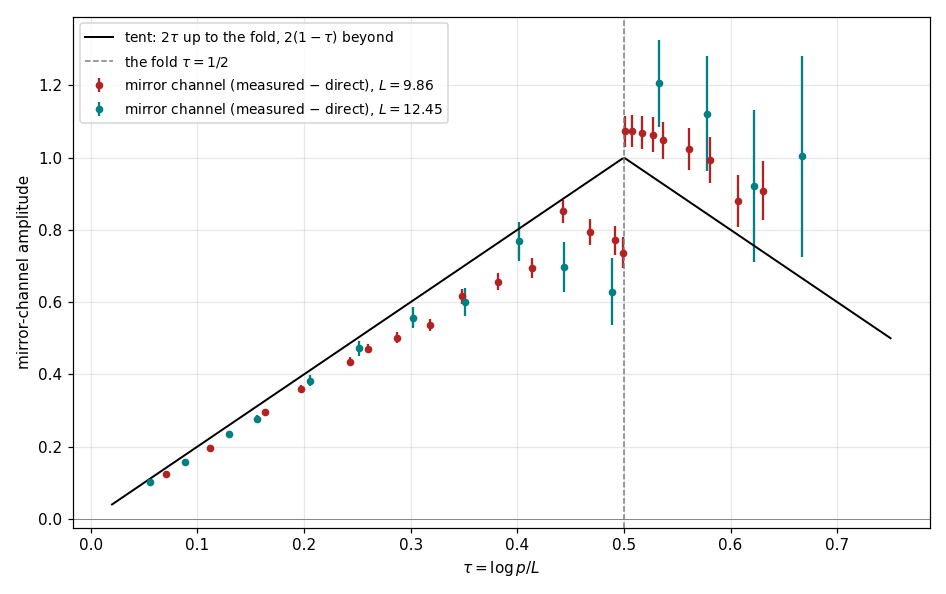
\includegraphics[width=0.82\textwidth]{fig_tent_en.png}
\caption{The mirror channel at two windows against the parameter-free
tent. The direct channel dies at the fold; the mirror channel peaks
there.}
\label{fig:tent}
\end{figure}

\section{The residual variance, decomposed}

The companion note's residual amplitude variance
$V_{\mathrm{res}}(L) = 0.163 \to 0.244$ (after stripping all
$p^k \le 300$) decomposes as follows. The unstripped tail, computed from
the measured $w(\tau)$ curve including its negative plateau, contributes
only $\sim 4.5\%$. Re-stripping with gap-interaction terms (the
transmission is gap-dependent) removes, placebo-corrected, a further
$0.074 \to 0.062$ --- $45\%$ to $25\%$ of the residual --- and lifts the
stripped core correlation to $0.984$. What remains grows linearly at
$0.035$ per unit $L$: within errors the \emph{CUE amplitude-variance
rate} ($0.036$ per unit $N$), at one tenth the magnitude (the
companion's ``one sixth'' referred to the raw, undecomposed residual). The zero gas
carries an intrinsic noise component that beats at the random-matrix
tempo but at a whisper.

\section{Synthesis and open problems}

The measured response theory of the zero gas now reads: each prime wave
enters at unit amplitude and is split, conserving amplitude, between
transmission and zero displacement ($\sqrt{w} + (\beta/2)v = 1$); the
medium is lossless, with a Bragg mirror at the Riemann--Siegel fold whose
observed position is shifted to $0.40$ by the measured, logarithmically
growing thermal jitter, with standing-wave dephasing of measured scale
$4.11$; the ideal structure factor is the fold's pair-counting
arithmetic; beyond the fold the response is carried entirely by the
functional equation's mirror sum, whose interference channel is a tent
peaked at the fold; and the last residue of randomness beats at the CUE
rate at one tenth amplitude.

Open problems: (1) the exact tent normalization from the classical
shifted-moment main terms, including the $\chi$-side; (2) the mapping of
the pointwise mirror channel to the max-channel plateau $B = -0.16$
(sign and size); (3) partial-reflection dressing $r(\tau)$ below the
Bragg condition; (4) a derivation of $\beta$; (5) the distribution (not
just variance) of the intrinsic core --- is it GUE?; (6) universality:
does the same response theory, with the same constants, hold for
Dirichlet $L$-functions?

\section*{Reproducibility}

All measurements are scripts 62--78 in
\url{https://github.com/azizran/deney} (directory \texttt{qm\_riemann/}),
runnable from the stored datasets; the dated research log records the
failed intermediate models alongside the results.

\section*{Acknowledgements}

Computational assistance, literature search and drafting: Claude
(Anthropic). Errors are the author's.

\begin{thebibliography}{9}

\bibitem{BCHB85} R.~Balasubramanian, J.~B.~Conrey, D.~R.~Heath-Brown,
\emph{Asymptotic mean square of the product of the Riemann zeta-function
and a Dirichlet polynomial}, J. reine angew. Math. \textbf{357} (1985),
161--181.

\bibitem{Berry88} M.~V.~Berry, \emph{Semiclassical formula for the number
variance of the Riemann zeros}, Nonlinearity \textbf{1} (1988), 399--407.

\bibitem{GHK07} S.~M.~Gonek, C.~P.~Hughes, J.~P.~Keating, \emph{A hybrid
Euler--Hadamard product for the Riemann zeta function}, Duke Math. J.
\textbf{136} (2007), 507--549.

\bibitem{OdlyzkoTables} A.~M.~Odlyzko, \emph{Tables of zeros of the
Riemann zeta function},
\url{https://www-users.cse.umn.edu/~odlyzko/zeta_tables/}.

\bibitem{companion1} U.~Sezen, \emph{The joint law of zero gaps and local
maxima of Hardy's $Z$-function}, draft (2026), same repository.

\bibitem{companion2} U.~Sezen, \emph{The prime-wave anatomy of the
gap--amplitude law for Riemann zeros}, draft (2026), same repository.

\end{thebibliography}

\end{document}
